\chapter{Generator Prompt Ablation Study}
\label{sec:ablation_edge}

Prompt engineering has emerged as a critical technique for optimizing large language model (LLM) performance on domain-specific tasks. To systematically evaluate the effectiveness of various prompting strategies for automated causal loop diagram generation, we conducted an ablation study comparing nine prompt variants across three causal loop diagrams.

\section{Experimental Design}

We evaluated nine prompt variants across three ground-truth causal loop diagrams:
\begin{itemize}[noitemsep]
    \item \textbf{CLD 1}: Depressive Symptoms in response to stressors (34 edges)
    \item \textbf{CLD 2}: Social Norms and obesity prevalence (12 edges)
    \item \textbf{CLD 3}: Emergency Department (66 edges)
\end{itemize}

All experiments used GPT-4.1 as the generator model with consistent hyperparameters (temperature=0.7, top\_p=1.0). Performance was measured using the F1 score, which balances precision and recall in edge discovery.

\section{Prompt Engineering Techniques}

Table~\ref{tab:prompt_techniques} presents a classification matrix of prompt engineering techniques employed in each variant, based on established literature.

\begin{table}[H]
\centering
\caption{Prompt Engineering Techniques Classification Matrix}
\label{tab:prompt_techniques}
\small
\begin{tabular}{@{}lccccc@{}}
\toprule
\textbf{Prompt} & \textbf{CoT\textsuperscript{1}} & \textbf{Few-Shot\textsuperscript{2}} & \textbf{Role\textsuperscript{3}} & \textbf{Decomp\textsuperscript{4}} & \textbf{RAG\textsuperscript{5}} \\
\midrule
Nitai\_A & & \checkmark & \checkmark & & \\
Nitai\_B & \checkmark & \checkmark & \checkmark & \checkmark & \\
Nitai\_C & \checkmark\checkmark & \checkmark\checkmark & \checkmark & \checkmark & \\
Nitai\_E & \checkmark\checkmark & \checkmark & \checkmark & \checkmark & \checkmark\checkmark \\
Rick\_A & & \checkmark & \checkmark\checkmark & & \\
Rick\_B & \checkmark & \checkmark\checkmark & \checkmark\checkmark & \checkmark\checkmark & \\
Cillian\_B & & \checkmark & \checkmark & \checkmark & \\
Cillian\_C & & \checkmark & \checkmark & \checkmark\checkmark & \\
Current & & \checkmark & & & \\
\bottomrule
\end{tabular}
\vspace{0.2cm}

\raggedright
\footnotesize
\textsuperscript{1}Chain-of-Thought~\cite{wei2022chain}; \textsuperscript{2}Few-Shot Learning~\cite{brown2020language}; \textsuperscript{3}Role Prompting; \textsuperscript{4}Task Decomposition; \textsuperscript{5}RAG with mandatory citations.\\
\vspace{0.1cm}
\textit{Legend:} \checkmark = basic; \checkmark\checkmark = strong implementation
\end{table}

\textbf{Key Prompt Distinctions:}
\begin{itemize}[noitemsep]
    \item \textbf{Nitai variants}: Progressive complexity from baseline (A) to Chain-of-Thought reasoning (B, C), culminating in RAG-augmented prompting (E). In the final experiments, Nitai\_C uses three relationship types (\texttt{POSITIVE}, \texttt{NEGATIVE}, \texttt{NONE}).
    \item \textbf{Rick variants}: Emphasis on academic rigor and system dynamics best practices. Rick\_B features comprehensive systematic decomposition with explicit confounding analysis.
    \item \textbf{Cillian variants}: Cillian\_B employs intervention-based framing. Cillian\_C uses hypothesis testing with definition-strict evaluation.
    \item \textbf{Current}: Minimal baseline control with basic prompting.
\end{itemize}

\section{Results}

\begin{figure}[H]
    \centering
    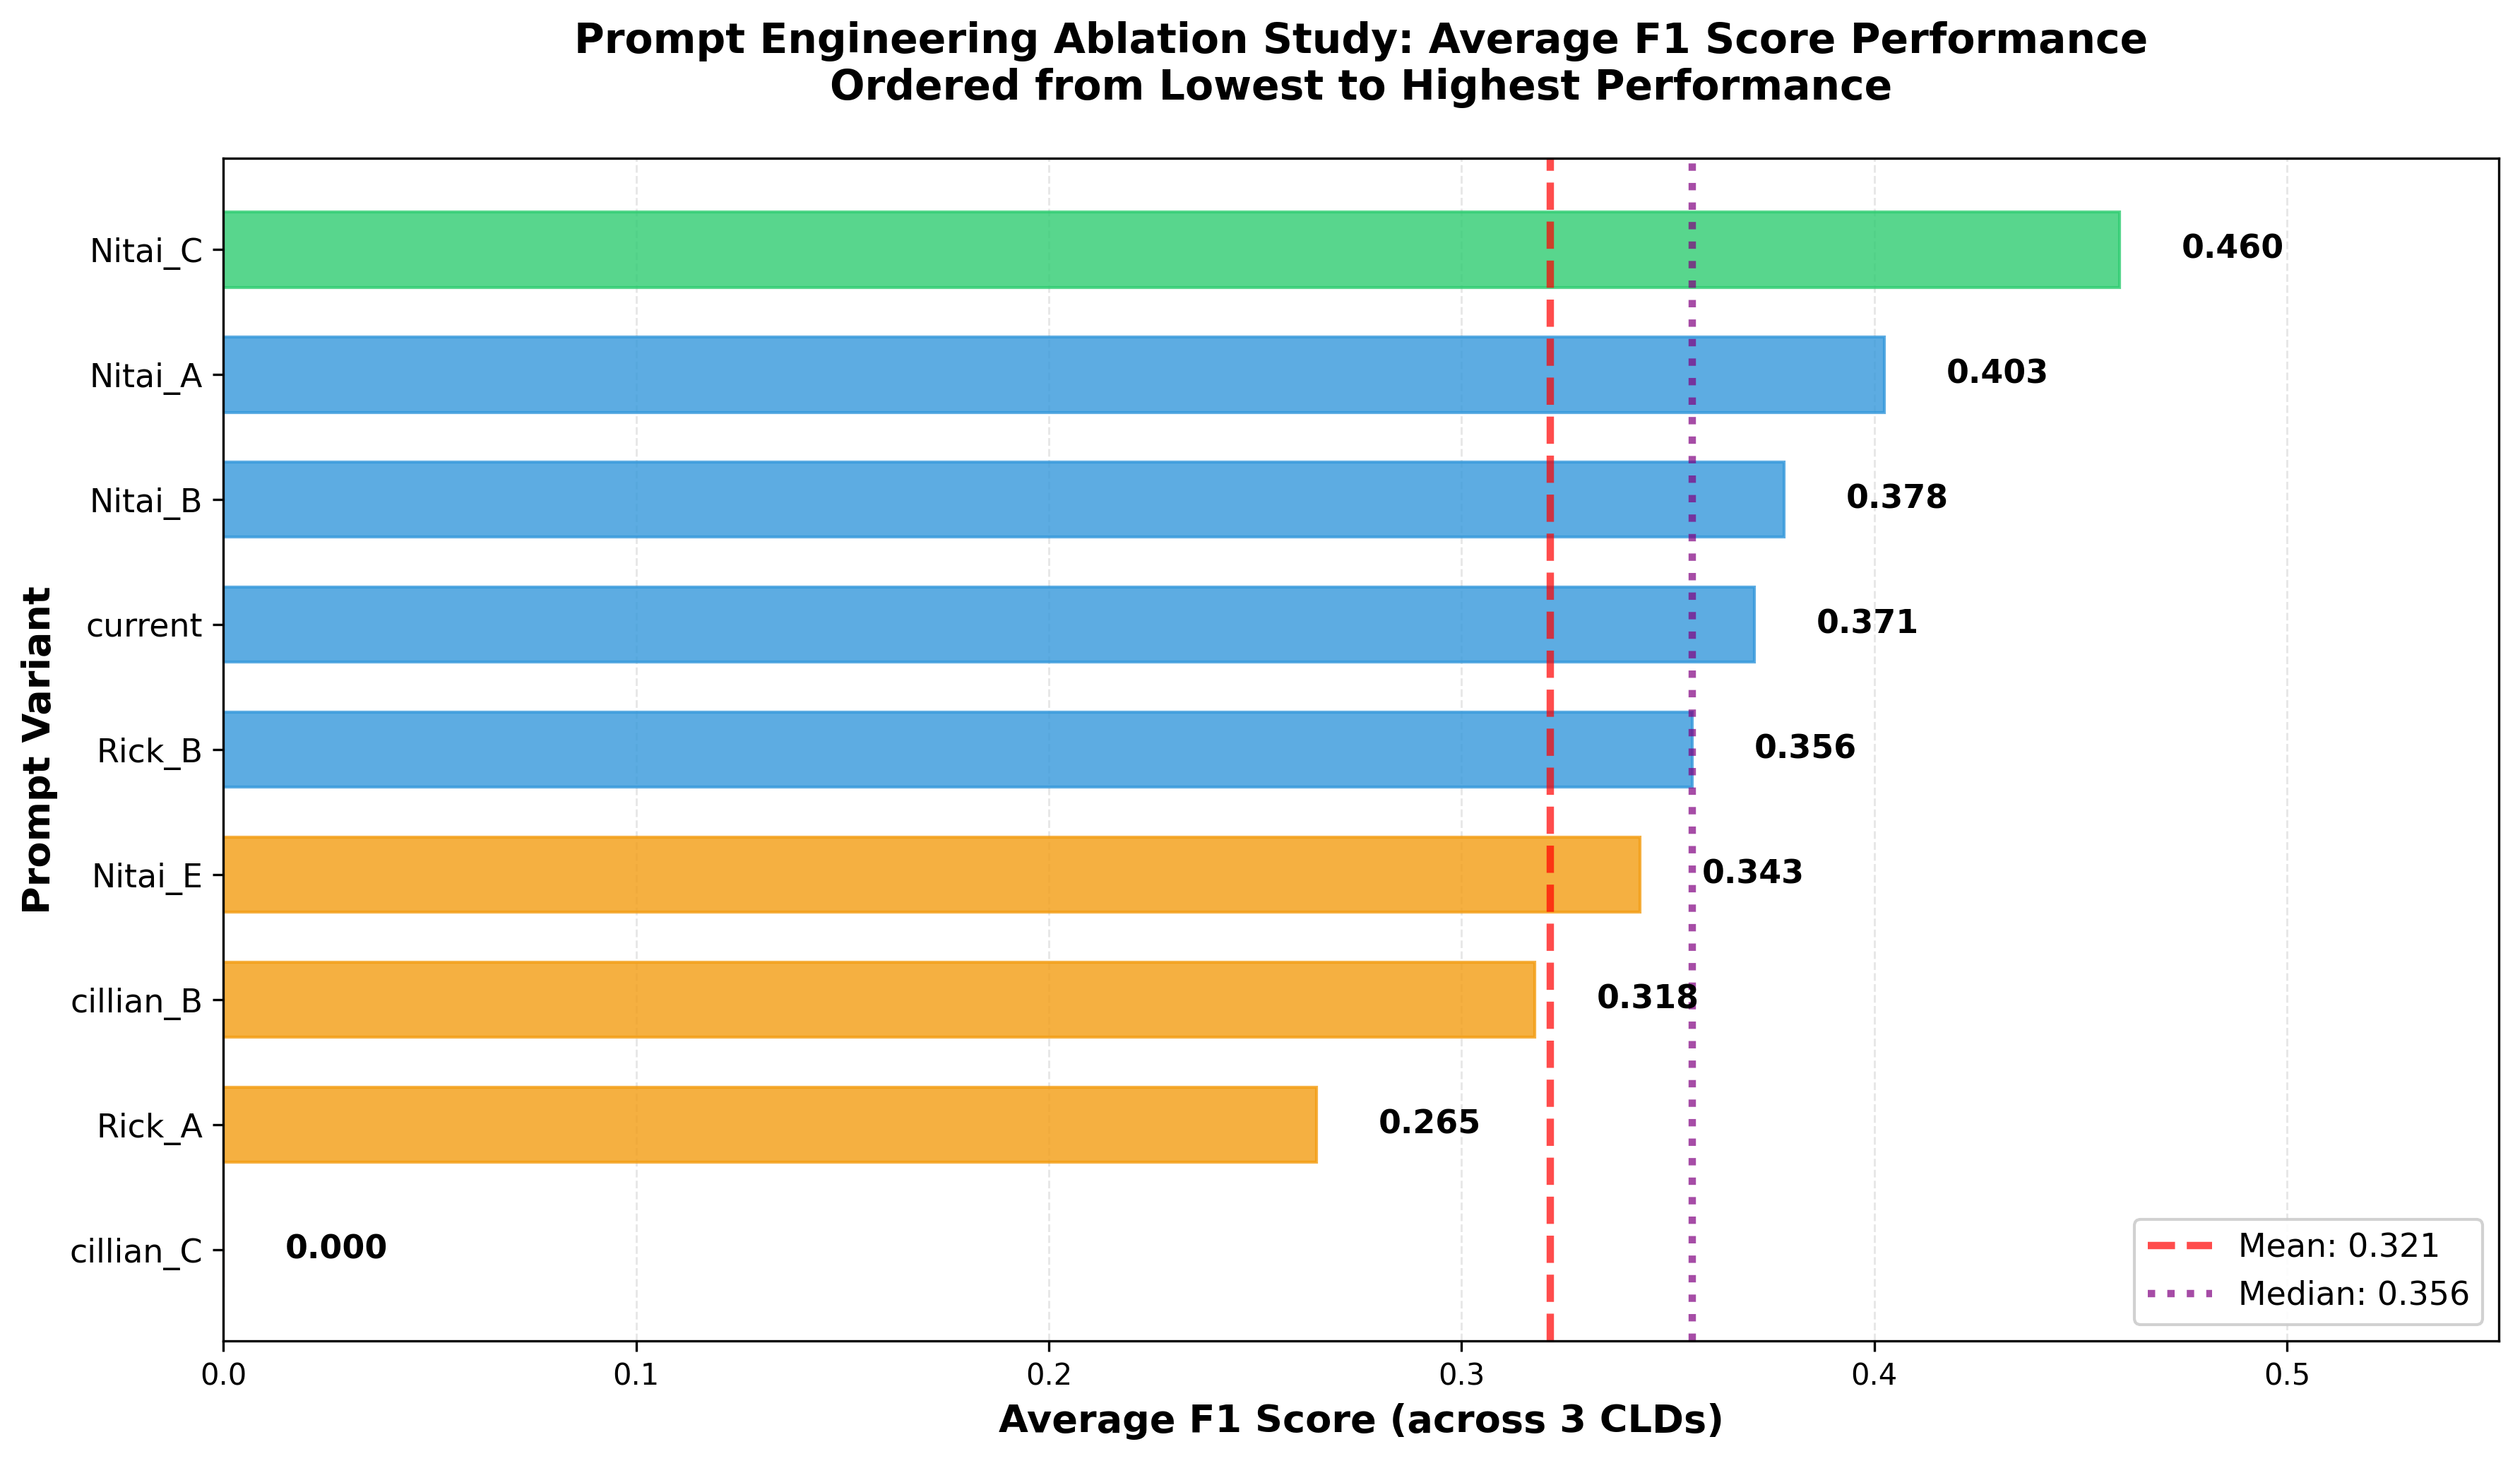
\includegraphics[width=0.95\textwidth]{Figures/edge_ablation_f1_ordered.png}
    \caption[Average F1 by prompt]{Average F1 scores for prompt variants across three CLDs, ordered from lowest to highest. Nitai\_C achieved highest performance (F1=0.460). Colour coding: green (F1 $\geq$ 0.45), blue (0.35--0.45), orange (0.25--0.35), red ($<$0.25).}
    \label{fig:ablation_f1_ordered}
\end{figure}

\begin{table}[H]
\centering
\caption{F1 Scores by Prompt Variant and Causal Loop Diagram}
\label{tab:f1_scores}
\begin{tabular}{@{}lcccc@{}}
\toprule
\textbf{Prompt} & \textbf{CLD 1} & \textbf{CLD 2} & \textbf{CLD 3} & \textbf{Average} \\
\midrule
Nitai\_C & 0.591 & 0.204 & 0.583 & \textbf{0.460} \\
Nitai\_A & 0.590 & 0.218 & 0.400 & 0.403 \\
Nitai\_B & 0.588 & 0.092 & 0.455 & 0.378 \\
Current & 0.588 & 0.239 & 0.286 & 0.371 \\
Rick\_B & 0.444 & 0.186 & 0.438 & 0.356 \\
Nitai\_E & 0.438 & 0.207 & 0.385 & 0.343 \\
Cillian\_B & 0.515 & 0.152 & 0.286 & 0.318 \\
Rick\_A & 0.380 & 0.145 & 0.269 & 0.265 \\
Cillian\_C & 0.000 & 0.000 & 0.000 & 0.000 \\
\bottomrule
\end{tabular}
\end{table}

\section{Key Findings}

\textbf{Overall Performance:}
\begin{itemize}[noitemsep]
    \item \textbf{Best Performance}: Nitai\_C achieved the highest average F1 score (0.460), differing from others in multiple dimensions (dual-level CoT, relationship taxonomy, examples).
    \item \textbf{Performance Range}: Range of 0.195 between best (0.460) and second-worst (0.265) performers. Mean F1 = 0.321, SD = 0.132.
\end{itemize}

\textbf{CLD-Specific Patterns:}
\begin{itemize}[noitemsep]
    \item \textbf{CLD 2 Challenge}: All variants performed worst on CLD 2 (Social Norms), with F1 scores 0.00--0.24.
    \item \textbf{High Variance}: Within-prompt SD across CLDs ranged 0.18--0.25, indicating sensitivity to problem characteristics.
\end{itemize}

\textbf{Technique-Specific Observations:}
\begin{itemize}[noitemsep]
    \item \textbf{RAG Trade-off}: Nitai\_E (mandatory citations) showed 25\% lower performance than Nitai\_C, suggesting strict citation requirements limit valid relationship discovery.
    \item \textbf{Complete Failure}: Cillian\_C's zero performance indicates overly restrictive definition-grounded evaluation can be counterproductive.
\end{itemize}

\section{Interpretation}

The progression Nitai\_A $\rightarrow$ Nitai\_B $\rightarrow$ Nitai\_C demonstrates incremental performance gains with Chain-of-Thought, achieving 14\% improvement over baseline. This supports Wei et al.'s~\cite{wei2022chain} findings that explicit reasoning steps enhance complex task performance.

Rick\_B (F1=0.356), employing systematic decomposition, underperformed Nitai\_C's CoT approach by 23\%, suggesting decomposition strategies may be less effective when tasks require holistic pattern recognition rather than sequential problem solving.

\section{Limitations}

\begin{itemize}[noitemsep]
    \item \textbf{Sample Size}: Only three CLDs limits generalizability.
    \item \textbf{Single Run}: Each variant tested once per CLD, preventing statistical significance testing.
    \item \textbf{Model Specificity}: Results apply to GPT-4.1; patterns may differ for other LLMs.
    \item \textbf{Prompt Authorship}: Different variants designed by different researchers, introducing potential confounding.
\end{itemize}


